\subsection{Lab5: Modulación BPSK en GRC}

%*********************
\begin{frame}{}

\pgfdeclareimage[width=\paperwidth,height=\paperheight]{bg}{imagenes/fondo_lab}
\setbeamertemplate{background}{\pgfuseimage{bg}}

\bfseries{\textrm{\LARGE Lab5\\ \Large Modulación BPSK en GRC}}
\raggedright
\end{frame}
%*********************

%--------------------------

\begin{frame}{Modulación BPSK en GRC}


\pgfdeclareimage[width=\paperwidth,height=\paperheight]{bg}{imagenes/fondo3}
\setbeamertemplate{background}{\pgfuseimage{bg}}


En esta práctica se hace uso de la modulación de desplazamiento de fase de 2 símbolos. Es el más sencillo de todos, puesto que solo emplea 2 símbolos, con 1 bit de información cada uno. Es también la que presenta mayor inmunidad al ruido, puesto que la diferencia entre símbolos es máxima (180º). Dichos símbolos suelen tener un valor de salto de fase de 0º para el 1 y 180º para el 0, como se muestra en un diagrama de constelación.
  

\end{frame}
%---------------------------

\begin{frame}{Modulación BPSK en GRC}

\begin{figure}
  \centering
   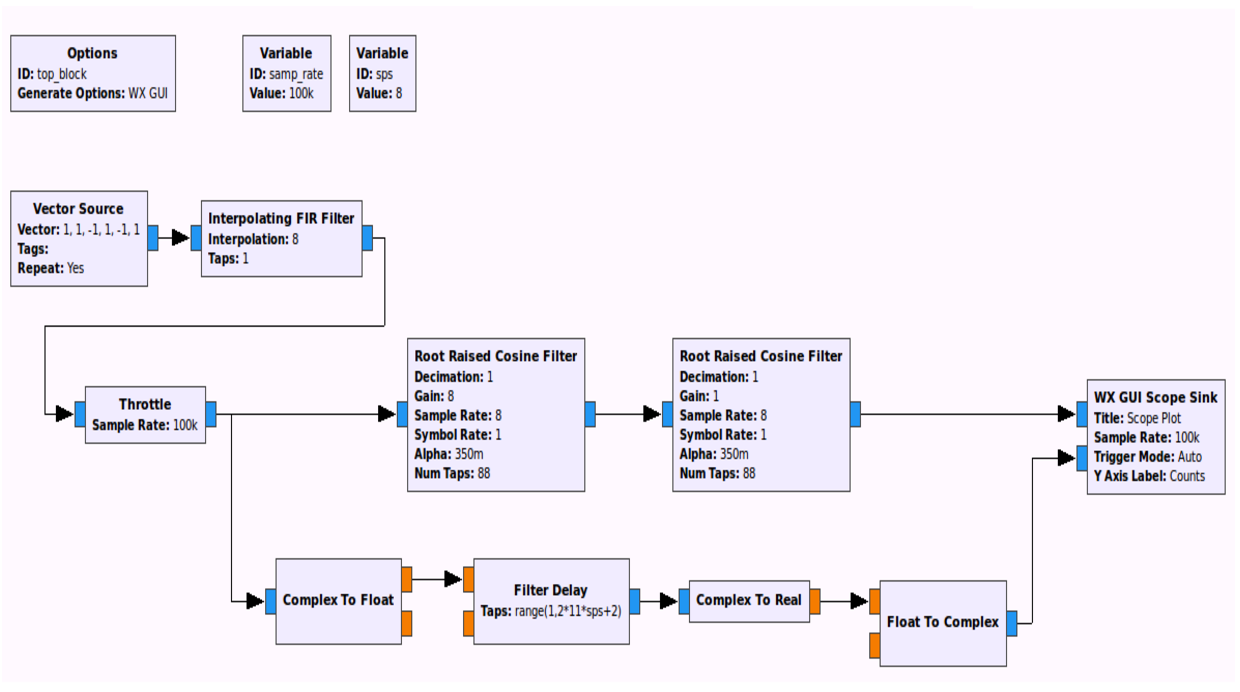
\includegraphics[width=\textwidth]{parte1/lab5/pdf/lab5_1.pdf}
  \end{figure}
  
\end{frame}
%------------------------

\begin{frame}{Modulación BPSK en función del tiempo}
\begin{figure}[H]
\centering
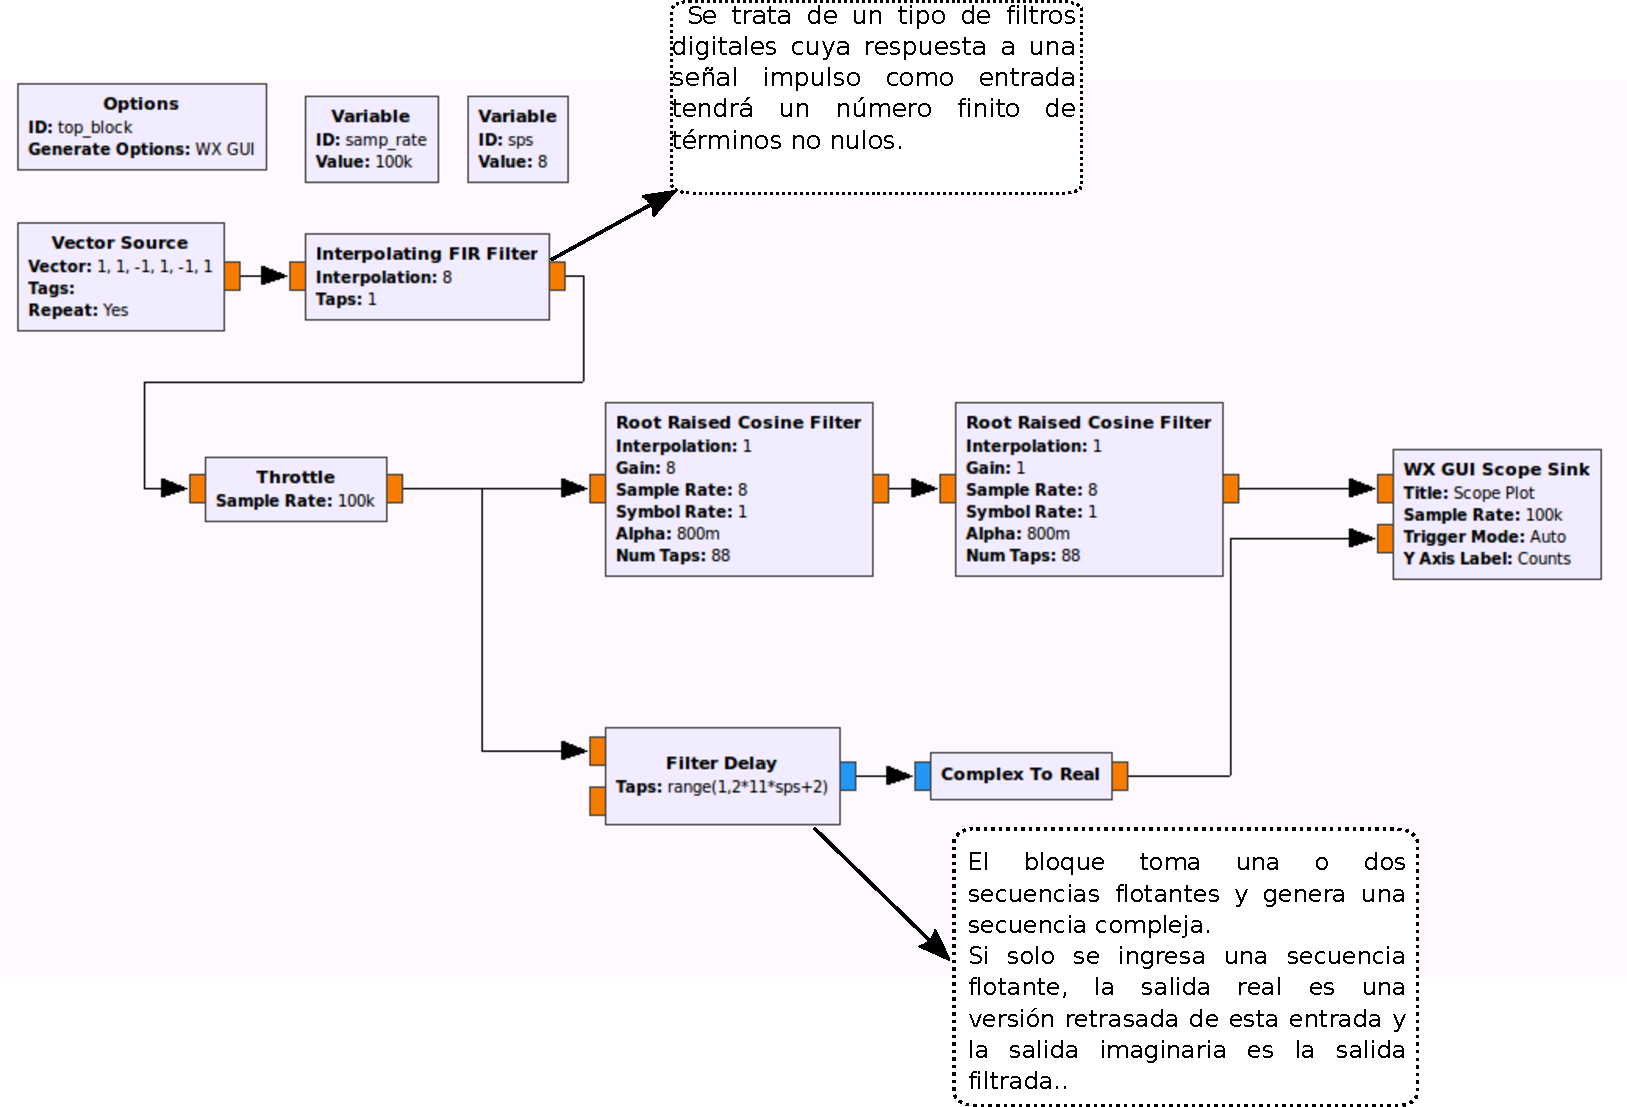
\includegraphics[width=.7\textwidth]{parte1/lab5/pdf/lab5_2.pdf}
\end{figure}
Convierte el flujo de datos digital en señal analógica de banda base (muestreada) utilizando el filtro FIR de interpolación.
\end{frame}
%------------------------

\begin{frame}{Modulación BPSK en GRC}
\begin{figure}[H]
\centering
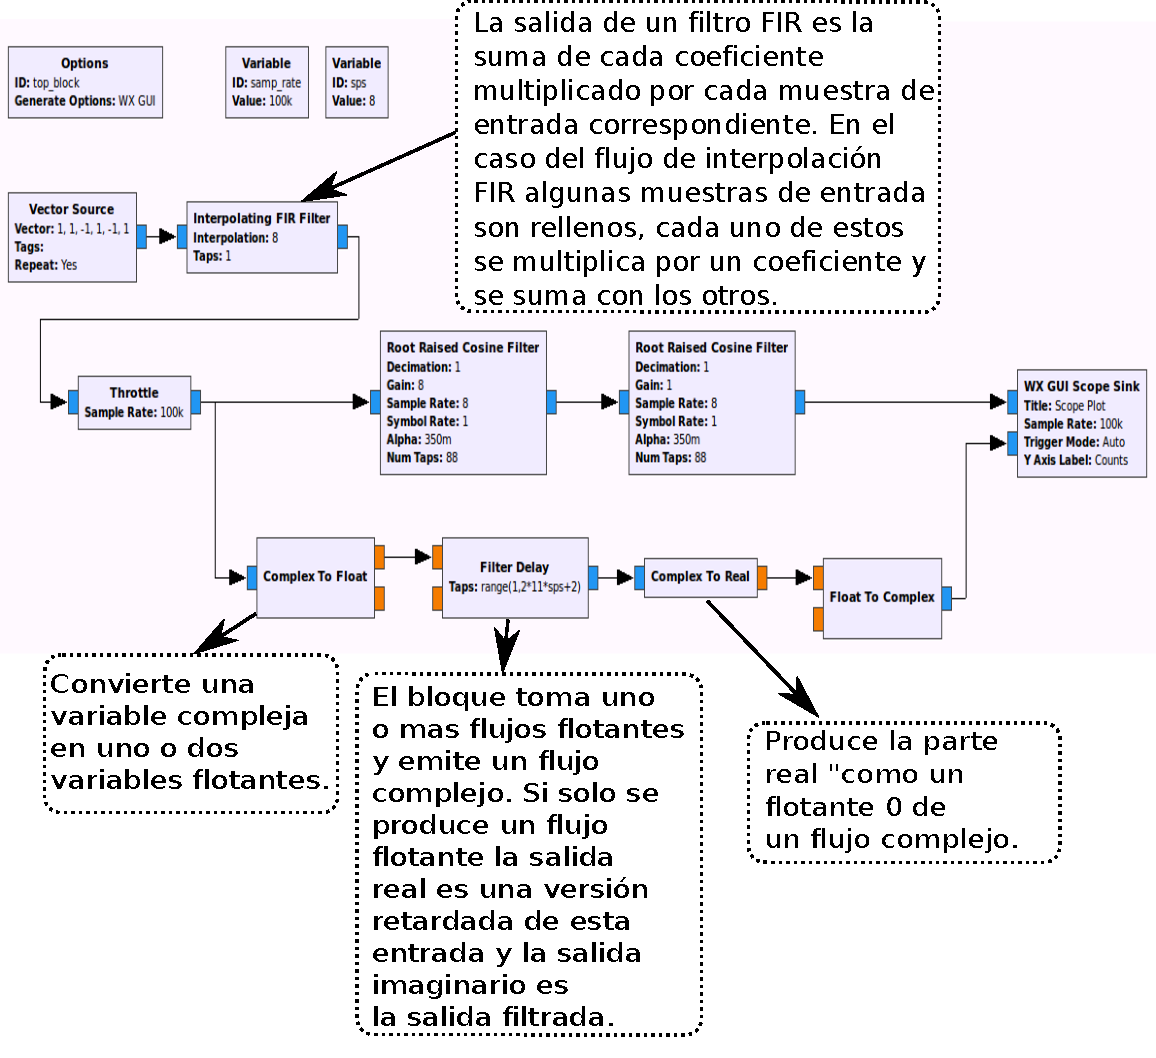
\includegraphics[width=.7\textwidth]{parte1/lab5/pdf/lab5_3.pdf}
\end{figure}
\end{frame}
%------------------------

\begin{frame}{Modulación BPSK en función del tiempo}
\begin{figure}[H]
\centering
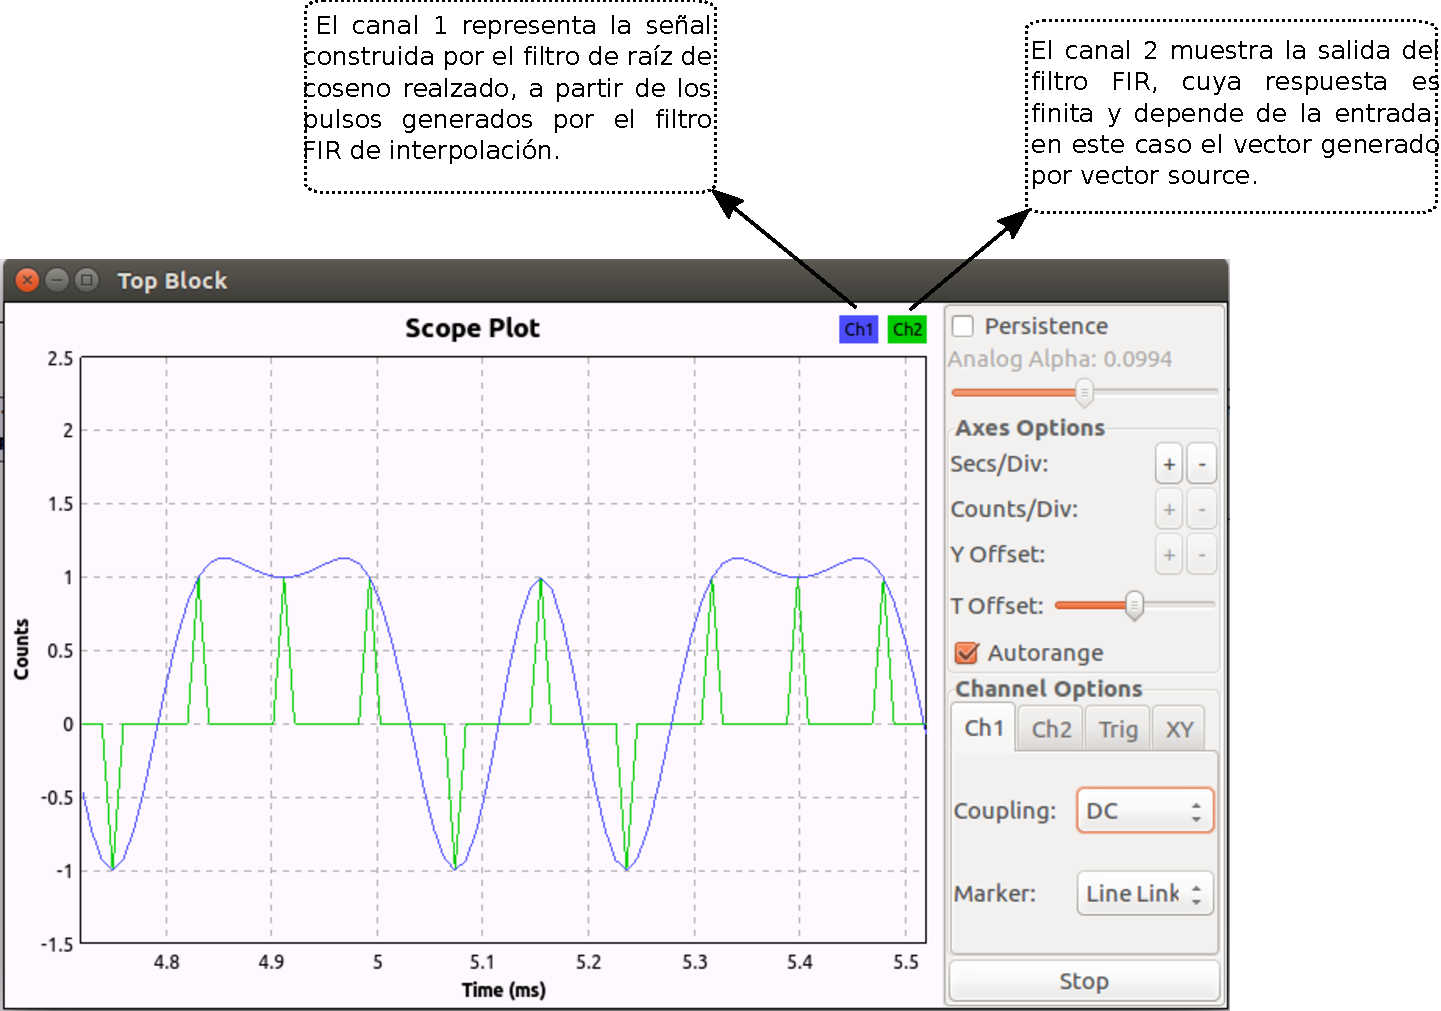
\includegraphics[width=.8\textwidth]{parte1/lab5/pdf/lab5_4.pdf}
\end{figure}
\end{frame}
%------------------------

\begin{frame}{Modulación BPSK en GRC}
\begin{figure}[H]
\centering
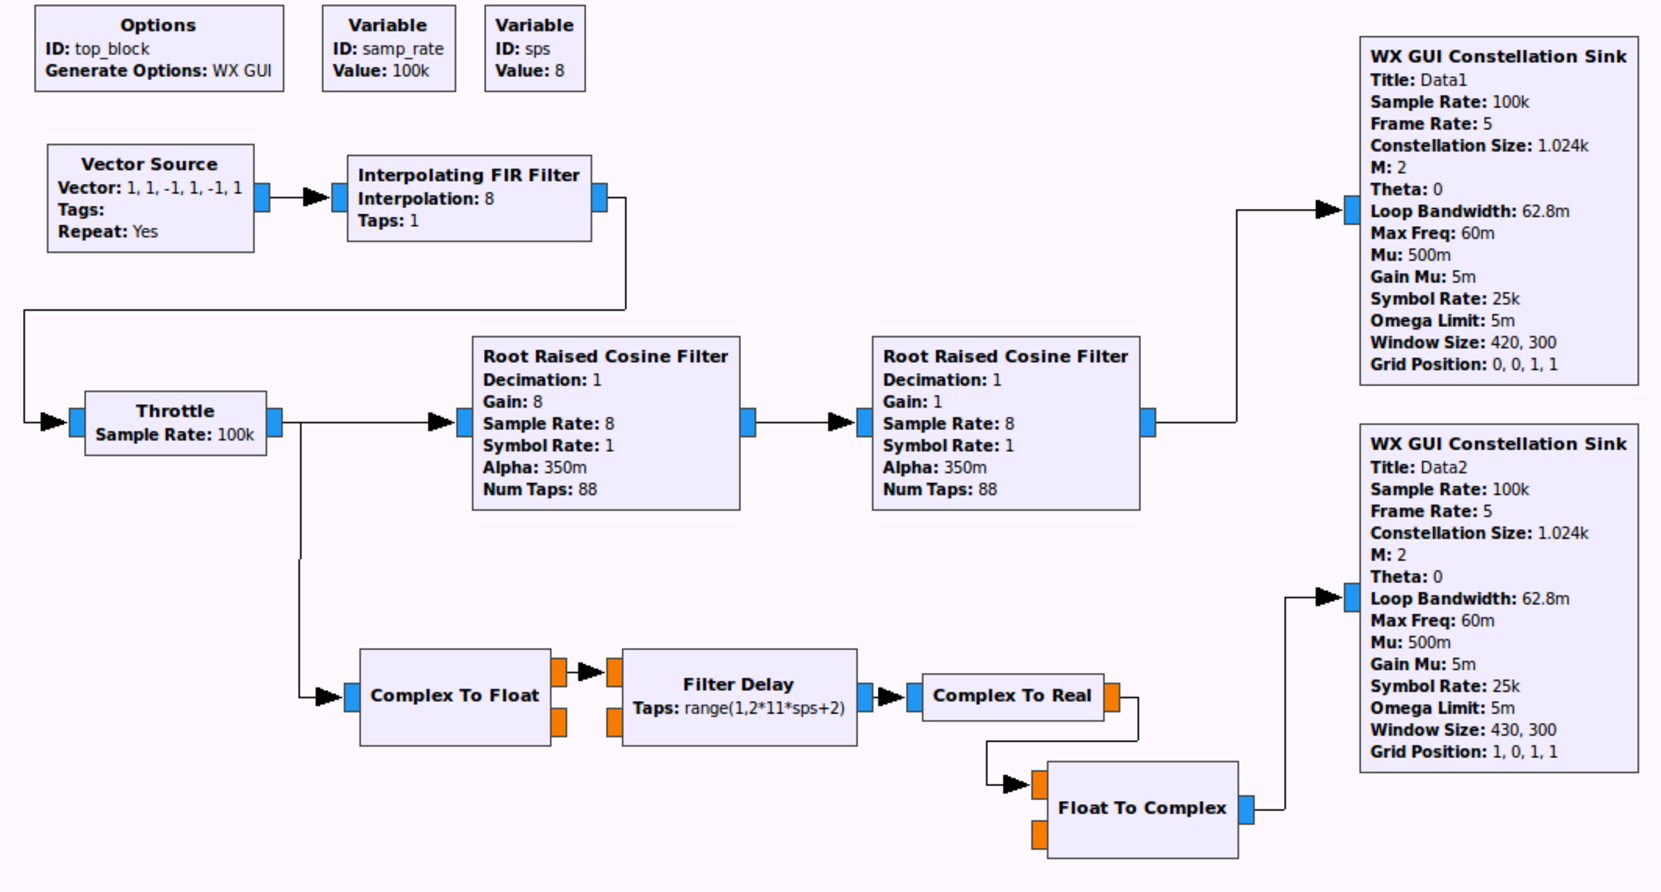
\includegraphics[width=\textwidth]{parte1/lab5/pdf/lab5_5.pdf}
\end{figure}
\end{frame}
%------------------------

\begin{frame}{Modulación BPSK en GRC}
\vspace{-8mm}
\begin{figure}[H]
\centering
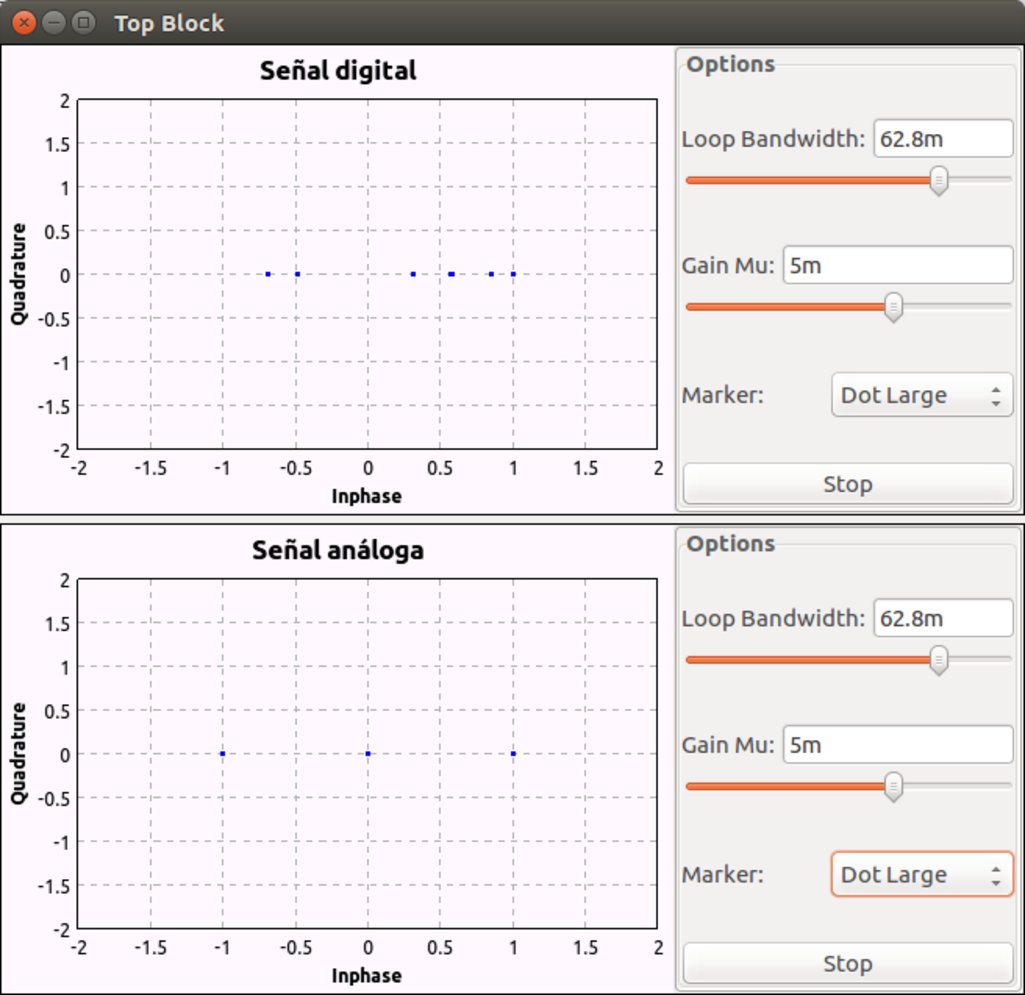
\includegraphics[width=.9\textwidth]{parte1/lab5/pdf/lab5_6.pdf}
\end{figure}
\tiny
Se deshabilita el bloque del osciloscopio WX GUI y se habilita el osciloscopio de constelaciones QT GUI , también se debe cambiar en el bloque Options: Generate options: WX GUI por QT GUI para que el bloque de constelaciones funcione.
\end{frame}
%------------------------

\begin{frame}{Constelación BPSK}
\begin{figure}[H]
\centering
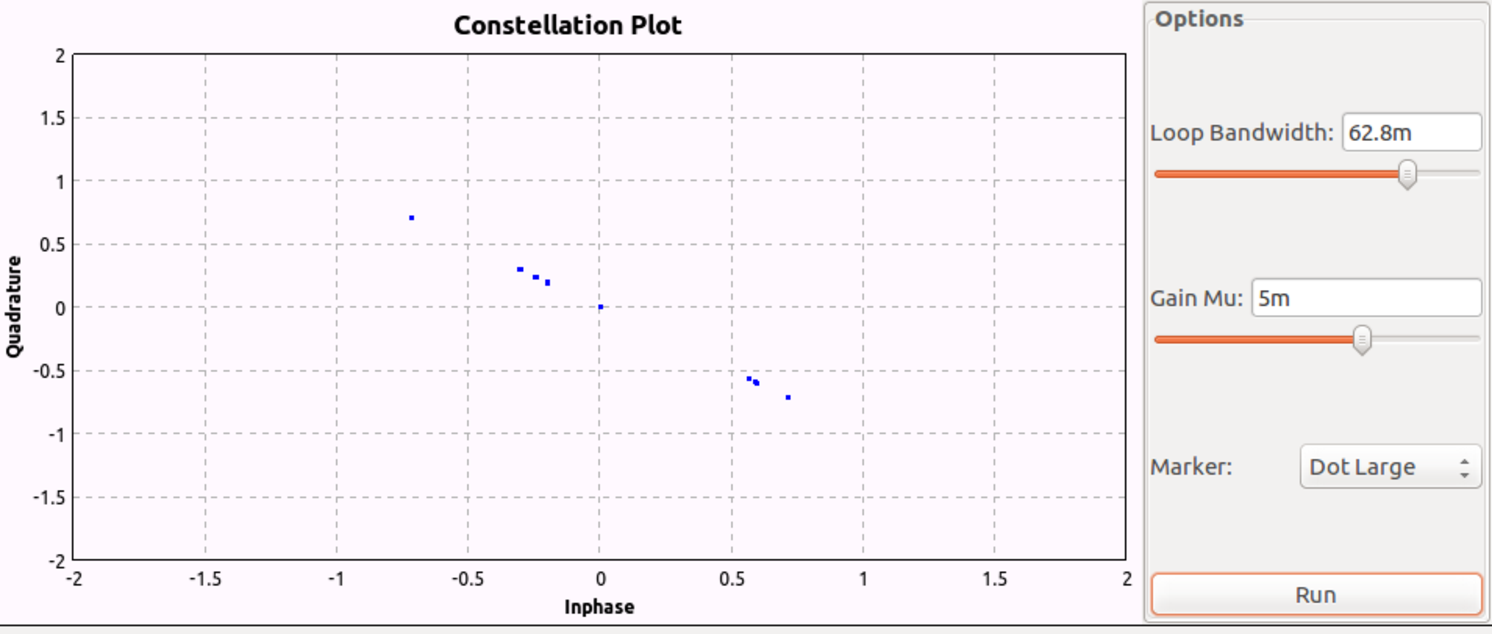
\includegraphics[width=\textwidth]{parte1/lab5/pdf/lab5_7.pdf}
\end{figure}
\end{frame}
%------------------------